\documentclass{beamer}

  %\usepackage{graphicx,eurofont}
  \usepackage{graphicx}
  \usepackage{color}
  \usepackage{bm,amssymb,amsmath}
  \usepackage{pst-all}
  \usepackage{harvard}
  %\usepackage{natbib}
  \usepackage{amsfonts}
  \usepackage{times}
  \usepackage{makeidx}
  \usepackage{mathrsfs}
  %\usepackage{rotating}
  \usepackage{mathpazo}
  \usepackage[draft,activate=pagevisible,deactivate=pageinvisible]{media9}
  %\usepackage{media9}
  \PassOptionsToPackage{pdfmark}{hyperref}\RequirePackage{hyperref}
  \addmediapath{/l/gentf1/Videos}, 
\setbeamersize{text margin left=2mm,text margin right=2mm}
%\setlength{\paperheight}{27.0cm}
%\setlength{\paperwidth}{29.7cm}
%\setlength{\textheight}{16.5cm}
%\setlength{\textwidth}{28.7cm}    
  
  \definecolor{burntorange}{RGB}{255,97,0}
  \definecolor{violet}{RGB}{105,20,200}
  \definecolor{royalblue}{RGB}{0,137,255}
%  \definecolor{mygreen}{RGB}{0,120,0}
  \newrgbcolor{myyellow}{1.0 1.0 0.5}
  \newrgbcolor{mygreen}{0 0.6 0.3}
  \newrgbcolor{myred}{0.9 0 0.1}
  \newrgbcolor{mymidblue}{0 0.2 0.7}
  \newrgbcolor{mypurple}{0.4 0 0.9}
  \newrgbcolor{dred}{0.5 0 0.1}
  \newrgbcolor{dblue}{0.1 0.0 0.6}
  \newrgbcolor{lightblue}{0.15 0.5 0.80}
  \newrgbcolor{white}{1. 1. 1.}
  \newrgbcolor{grey}{0.5 0.5 0.5}
  \newrgbcolor{whiteblue}{.80 .80 1.}

  \newenvironment{notes}
  {\color{grey} }

\newcommand\fV{ f_{V,i}}
\newcommand\fH{ f_{V,h}}
\newcommand{\vect}[1]{{{\mbox{\boldmath $#1$}}}}%also makes bold Greek letters
\newcommand\barg{{\overline{\gamma}}}
\newcommand\eB{{\langle e_{\rm B}\rangle}}
\newcommand\eK{{\overline{e_{\rm K}}}}
\newcommand\ESK{E_{\rm kin}}
\newcommand\EST{E_{\rm th}}
\newcommand\ESN{E_{\sigma}}
\newcommand\cs{ c_{\rm s}}
\newcommand\cp{ c_{\rm p}}
\newcommand\cv{ c_{\rm v}}
\newcommand\Rm{{\rm Rm} }
\newcommand\Rey{{\rm Re} }
\newcommand\Pm{{\rm Pm} }
  \newcommand\bmt[1]{{\mbox{\boldmath $#1$}}}
  \newcommand\average[1]{{\langle #1 \rangle}} %volume average
  \newcommand\mean[1]{\overline{#1}}         %ensemble average
  \newcommand{\cold}{{_{\rm c}}}
  \newcommand{\w}{{_{\rm w}}}
  \newcommand{\h}{{_{\rm h}}}
  \newcommand{\tphi}{{\Phi}}  %ensemble-averaged philling factor
  \newcommand{\rms}{{_{\rm rms}}}
  \newcommand{\Gyr}{\,{\rm Gyr}}
  \newcommand{\g}{\,{\rm g}}
  \newcommand{\Myr}{\,{\rm Myr}}
  \newcommand{\mesh}{{_{\Delta x}}}			%resolution
  \newcommand{\SN}{_{\rm SN}}     				%supernova
  \newcommand\sfrac[2]{{\textstyle{\frac{#1}{#2}}}}
  \newcommand{\mathbfss}[1]{\textbf{\textsf{#1}}}
  \newcommand{\sound}{{_{\mathrm{s}}}}  			%sound
  %
  %       UNITS
  %
  \newcommand{\cm}{\,{\rm cm}}
  \newcommand{\mm}{\,{\rm mm}}
  \newcommand{\cmcube}{\,{\rm cm^{-3}}}
  \newcommand{\dyn}{\,{\rm dyn}}
  \newcommand{\erg}{\,{\rm erg}}
  \newcommand{\Jy}{\,{\rm Jy}}
  \newcommand{\Jyb}{\,{\rm Jy/beam}}
  \newcommand{\km}{\,{\rm km}}
  \newcommand{\kms}{\,{\rm km\,s^{-1}}}
  \newcommand{\mJy}{\,{\rm mJy}}
  \newcommand{\mJyb}{\,{\rm mJy/beam}}
  \newcommand{\K}{\,{\rm K}}
  \newcommand{\sh}{\,{\rm shock}}
  \newcommand{\kpc}{\,{\rm kpc}}
  \newcommand{\Mpc}{\,{\rm Mpc}}
  \newcommand{\mG}{\,{\rm mG}}
  \newcommand{\mkG}{\,\mu{\rm G}}
  \newcommand{\MHz}{\, {\rm MHz}}
  \newcommand{\Msol}{\,{\rm M_\odot}}
  \newcommand{\p}{\,{\rm pc}}
  \newcommand{\radm}{\,{\rm rad\,m^{-2}}}
  \newcommand{\s}{\,{\rm s}}
  \newcommand{\yr}{\,{\rm yr}}
  \newcommand{\an}{{Astron.\ Nachr.}}
  \newcommand{\apj}{{ApJ}}
  \newcommand{\rmp}{{Rev.\ Mod.\ Phys.}}
  \newcommand{\Pra}{{\rm Pr}}
  \newcommand{\pre}{{\rm Ph.\ Rev.\ E.}}
  \newcommand{\prl}{{\rm Ph.\ Rev.\ L.}}
  \newcommand{\araa}{ARA\&A}
  \newcommand{\aj}{{AJ}}
  \newcommand{\aap}{{A{\&}A}}
  \newcommand{\apjl}{{ApJ Letters}}
  \newcommand{\mnras}{{MNRAS}}
  \newcommand{\jfm}{{J.\ Fluid Mech.}}    
\newcommand\uOl{\texttt{UP0r10sl}}
\newcommand\hOl{\texttt{HP0r10sl}}
\newcommand\hIl{\texttt{HP1r10sl}}
\newcommand\hIIl{\texttt{HP2r5sl}}
\newcommand\hVm{\texttt{HP5r8sm}}
\newcommand\hVmL{\texttt{HP5r8sm-L}}
\newcommand\hVl{\texttt{HP5r2sl}}
\newcommand\mOh{\texttt{MP0r10sh}}
\newcommand\mOIh{\texttt{MP0r5sh}}
\newcommand\mIIl{\texttt{MP2r5sl}}
\newcommand\mOl{\texttt{MP0r10sl}}
\newcommand\lOIh{\texttt{LP0r5sh}}
\newcommand\lOh{\texttt{LP0r10sh}}
\newcommand\lOl{\texttt{LP0r10sl}}
\newcommand\lIIl{\texttt{LP2r5sl}}
\newcommand\lVmS{\texttt{LP5r8sm-S}}
      \bibliographystyle{jphysicsB}
  \setbeamertemplate{bibliography item}[text]
%%
%%
%%
\author{ 
        {\footnotesize
         {Frederick Gent \inst{1,5}, Maarit K\"apyl\"a \inst{1,4,6}, 
         Mordecai-Mark Mac Low \inst{2},\\
         Nishant Singh \inst{3}
}}}
%
\title{\color{white}{The sporadic nature of small-scale dynamo in 
supernova-driven ISM turbulence and its effects on the large scale dynamo and galactic magnetic fields\vspace{0.5cm}
}}
%
\date{\color{white}\today -- Nordita astro seminar series}
%
\institute{\tiny{\color{white}
{$^1$ReSoLVE, Department of Computer Science, Aalto University, Espoo, Finland
\and
$^2$Department of Astrophysics, American Museum of Natural History, New York, USA
\and
$^3$Inter University Centre for Astronomy and Astrophysics, Pune, India
\and
$^4$Nordita, KTH Royal Institute of Technology \& Stockholm University, Hannes Alfv\'ens v\"ag 12, Stockholm, SE-11419, Sweden
\and
$^5$Department of Mathematics, Newcastle  University, Newcastle upon Tyne, UK
\and
$^6$Max-Planck-Institut f\"ur Sonnensystemforschung, G\"ottingen, Germany
}}}
%
%
%%%%%%%%%%%%%%%%%%%%%%%%%%%%%%%%%%%%%%%%%%%%%%%%%%%%%%%%%%%%%%%%%%%%%%%%%%%%%

\begin{document}

%----------------------------------------------------------------------------
% title slide with astronomical image background 
  {
  \usebackgroundtemplate
    {\hspace{-2.75cm}\vspace{-7.5cm}
     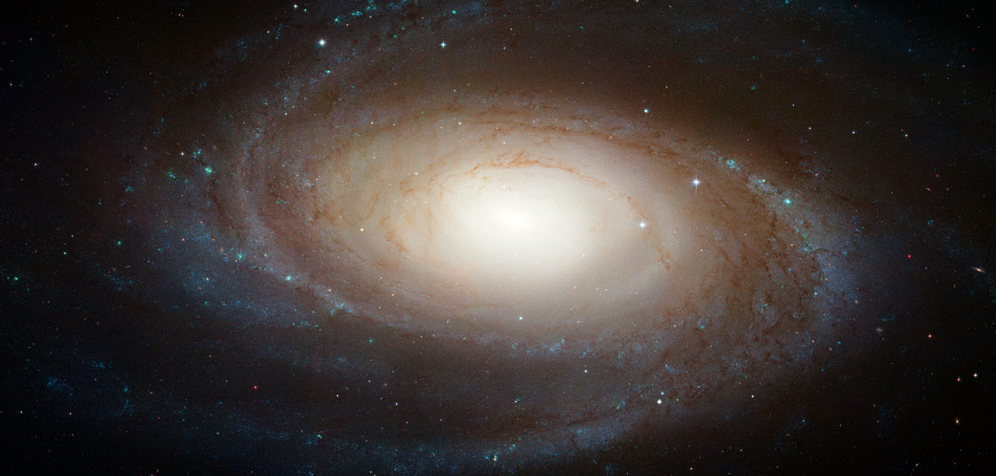
\includegraphics [width=1.35\paperwidth,height=\paperheight]
    {hs-2007-19_M81b.png} }
    \begin{frame}
      \maketitle{\white}
    \end{frame}
  }

%----------------------------------------------------------------------------
%%----------------------------------------------------------------------------
%
%  \section{Intro: Outline of simulations and presentation}
%
%----------------------------------------------------------------------------

  \subsection{Supernova modelling}

%------------------------------------------------------------------------
  \section{Supernova driven turbulence}
  \subsection{Our place in the Galaxy}
%------------------------------------------------------------------------
  \begin{frame}
    \frametitle{\colorbox{white}{Galactic scales}}
      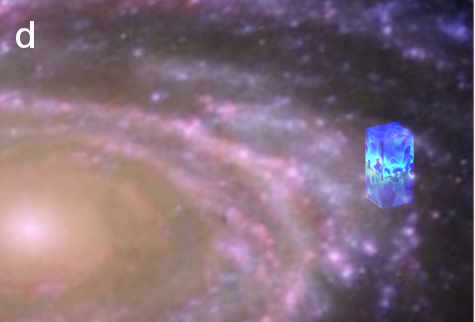
\includegraphics[trim=1.8cm 0cm -1cm 2cm,clip=true,width=1.15\textwidth]{spiralbox.png}
  %\begin{picture}(0,0)(0,0)
  %  \put(25,95){{\sf\bf{ Alpha Centauri -- 1 parsec 4 lightyears}}}
  %  \put(25,70){{\sf\bf{``Vacuum of space" -- 1 atom cm$^{-3}$ (air 10$^{22}$cm$^{-3}$)}}}
  %  \put(25,45){{\sf\bf{2 million cpu hours \quad  box: $1\times1\times2\kpc^3$ }}}
  %  \put(25,20){{\sf\bf{280 processors   \quad $256\times256\times560$ resolution }}}
  %\end{picture}
  \end{frame}

  \subsection{What does it take to get a galactic dynamo?} 
    \begin{frame}
      \frametitle{What does it take to get a galactic dynamo?}
    \begin{columns}
      \begin{column}[]{6.0cm}
       %\includemovie[autoplay]{6.0cm}{5.6cm}{rho.avi}
       %\includemedia[autoplay,width=6.0cm,height=5.6cm,activate=pagevisible,deactivate=pageinvisible]{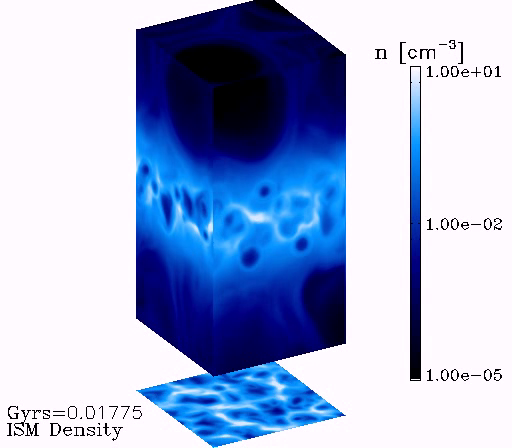
\includegraphics[width=6.0cm]{rho.avi.jpg}}{rho.avi}
       %\includemedia[width=6.0cm,height=5.6cm,activate=pagevisible,deactivate=pageinvisible,draft]{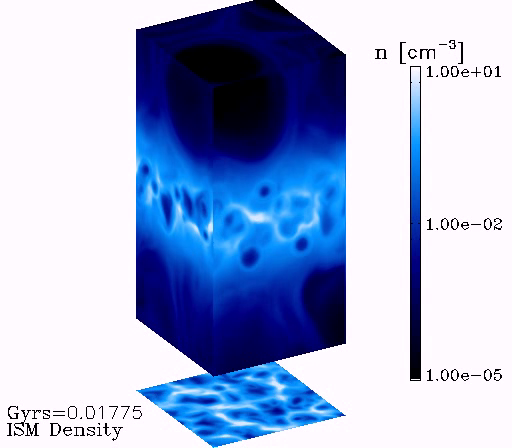
\includegraphics[width=6.0cm]{rho.avi.png}}{rho.avi}
       \includemedia[width=6.0cm,keepaspectratio,activate=pagevisible,addresource=rho.avi,final]{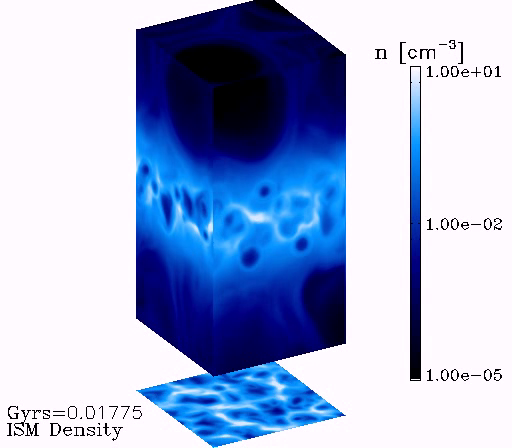
\includegraphics[]{rho.avi.png}}{rho.avi}
  
    {\footnotesize{gas density}}
      \end{column}
      \begin{column}[]{6.0cm}
       %\includemedia[width=6.0cm,height=5.6cm,activate=pagevisible,deactivate=pageinvisible,draft]{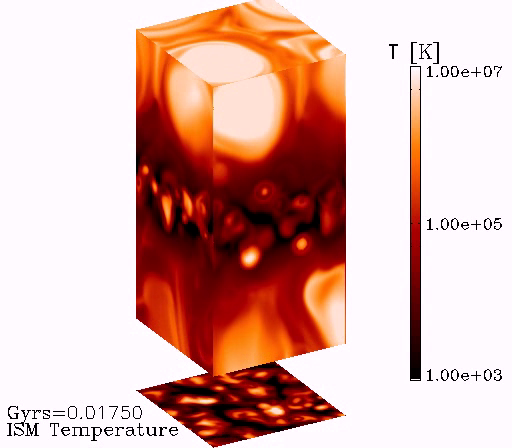
\includegraphics[width=6.0cm]{tt.avi.png}}{lnTT.avi}
       %\includemovie[autoplay]{6.0cm}{5.6cm}{lnTT.avi}
       \includemedia[width=6.0cm,height=5.6cm,activate=pagevisible,draft]{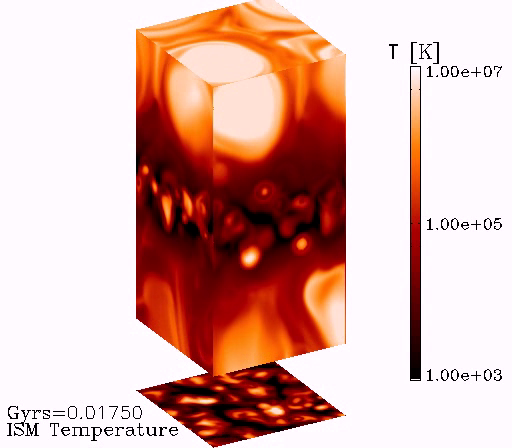
\includegraphics[]{tt.avi.png}}{tt.avi}

      {\footnotesize{temperature}}
      \end{column}
    \end{columns}
      \vspace{0.5cm}
      \centering{\footnotesize{\cite{Gent:2013a} }}
    \end{frame}
%----------------------------------------------------------------------------
%  \subsection{What does it take to get a galactic dynamo?} 
    \begin{frame}
      \frametitle{What does it take to get a galactic dynamo?}
    \begin{columns}
      \begin{column}[]{6.5cm}
       %\includemovie[autoplay]{6.5cm}{6.5cm}{e_b.avi}
      {\footnotesize{\cite{Gent:2013b}}}
      \end{column}
      \begin{column}[]{6.25cm}
      {\footnotesize{
      \begin{itemize}
        \item rotation, shear and turbulence - including vorticity
        \item SSD $\Rm\gtrsim20$ \cite{SBK02,HB04,Schober12,SBSW20}
        \item we get effective $\Rm\simeq30$ \cite{HSSFG17}
        \item shock turbulence suppress dynamo \cite{Haugen:2004M,FCSBKS11,FSBS14}?
        \item effect of baroclinicity -- increased vorticity, esp on smaller scales \cite{KGVS18,SF22}
	\item time -- over a gigayear
      \end{itemize}
       \vspace{-0.2cm}
      }}
      \end{column}
    \end{columns}
    \end{frame}
%----------------------------------------------------------------------------
    \begin{frame}
	    \begin{center}
      \frametitle{What does it take to get a galactic dynamo?}
       %\includemovie[autoplay]{12cm}{6.5cm}{videos/strat-ebTn.avi}
	    
{\footnotesize{5 Gyr to saturate LSD -- 4 pc model (1 pc 45 Million cpu hours to 1 Gyr)}}
	    \end{center}
    \end{frame}
%----------------------------------------------------------------------------
%----------------------------------------------------------------------------
  \subsection{equations}
%------------------------------------------------------------------------
    \begin{frame}
      \frametitle{Equations}
%----------------------------------------------------------------------------
  \begin{align}
  \label{eq:mass}
  \frac{D\rho}{Dt}\, = &
      \,- \nabla \cdot (\rho \bmt{u})\,
    +\nabla \cdot\zeta_D\nabla\rho,\\[0.5cm]
%----------------------------------------------------------------------------
  \label{eq:mom}
  \rho~\frac{D\bmt{u}}{Dt} \,= &~
    \nabla{\ESK\sigma}
    -\rho~\cs^2\nabla\left({s}/{\cp}+\ln\rho\right)
        \,-\rho~\nabla\Phi
        \,-\rho~Su_x\bm{\hat{y}}
    \\
    &+\vect{j}\times\vect{B}
        \,-\,2\bmt{\Omega}\times\bmt{u}
    +\nabla\cdot \left(2\rho\nu{\mathbfss W}\right)
    +\rho~\nabla\left(\zeta_{\nu}\nabla \cdot \vect{u} \right)
    \nonumber\\
    &+\nabla\cdot \left(2\rho\nu_6{\mathbfss W}^{(6)}\right)
  {-\vect u\vect{\nabla}\cdot\left(\zeta_D\vect{\nabla}\rho\right)},\nonumber\\[0.5cm]
%----------------------------------------------------------------------------
  \label{eq:ent}
    \rho T\frac{D s}{Dt} = &
    ~\EST\dot\sigma +\rho\Gamma_{\rm UV}
    -\rho^2\Lambda +\eta\mu_0\vect{j}^2 
    +2 \rho \nu\left|{\mathbfss W}\right|^{2}
    +\rho~\zeta_{\nu}\left(\nabla \cdot \vect{u} \right)^2
    \\
    &+\nabla\cdot\left(\zeta_\chi\rho T\nabla s\right)
    +\rho T\chi_6\nabla^6 s
    - \cv~T \left(\zeta_D\nabla^2\rho + \nabla\zeta_D\cdot\nabla\rho\right),\nonumber\\[0.5cm]
		    \label{eq:ind}
    \frac{\partial \vect{A}}{\partial t} = &
    ~\vect{u}\times\vect{B}
    +\eta\nabla^2\vect{A}
    +\eta_6\nabla^6\vect{A}
  \end{align}
%----------------------------------------------------------------------------
  \end{frame}
%----------------------------------------------------------------------------
  \subsection{Small scale dynamo in SN driven ISM turbulence?} 
    \begin{frame}
      \frametitle{Galaxy fluctuation dynamo growth rates}
    \begin{columns}
      \begin{column}[]{6.0cm}
       \begin{figure}
        \includegraphics[width=\textwidth]{ssdfigs/res-comp.pdf}
        \includegraphics[width=\textwidth]{ssdfigs/res-logcomp.pdf}
       \end{figure}
      \end{column}
      \begin{column}[]{5.8cm}
	       \begin{center}
            $\eta=10^{-4}$kpc km s$^{-1}$\vspace{0.5cm}
	    
$\nu=0$\vspace{0.5cm} 

Convergence for $\delta x\leq 1$ pc.\vspace{1cm} 
\begin{equation}\label{eq:barg}
\eB(t)=\eB(t_0)\exp[\barg(t-t_0)].
\end{equation}
	       \end{center}
      \end{column}
      \end{columns}
    \end{frame}
%----------------------------------------------------------------------------
    \begin{frame}
      \frametitle{ISM SSD multiphase structure}
       \begin{figure}
        \includegraphics[trim=1.0cm 0cm 0.5cm 0.3cm,clip=true,width=0.46\textwidth]{paperfigs/rh78.pdf}
        \includegraphics[trim=1.0cm 0cm 0.5cm 0.3cm,clip=true,width=0.46\textwidth]{paperfigs/tt78.pdf}
        \includegraphics[trim=1.0cm 0cm 0.5cm 0.3cm,clip=true,width=0.48\textwidth]{paperfigs/eB78.pdf}
       \end{figure}

    \end{frame}
%----------------------------------------------------------------------------
    \begin{frame}
      \frametitle{Magnetic energy growth rates and fractional volume}
Growth rate locally $\Gamma(\vect{x})$. 
Take the curl of Eq.~\eqref{eq:ind}, contract it with $\vect{B}\mu_0^{-1}$
%-----------------------------------------------------------------------------
  \begin{eqnarray}
  \label{eq:eB}
    \frac{\partial e_{\rm B}}{\partial t} &=&
    \vect{B}\cdot\nabla\times\left(\vect{u}\times\vect{B}
    +\eta\nabla^2\vect{A}\right)\mu_0^{-1}.
  \end{eqnarray}
Dividing by $e_{\rm B}$, the {\em relative} growth rate exponent at each instant in time 
%-----------------------------------------------------------------------------
  \begin{eqnarray}
  \label{eq:logeB}
    \Gamma (\vect{x})  &=&\frac{\vect{B}\cdot\nabla\times\left(\vect{u}\times\vect{B}
    +\eta\nabla^2\vect{A}\right)}{e_{\rm B}\mu_0},
  \end{eqnarray}
%-----------------------------------------------------------------------------
where $e_{\rm B} \propto \exp(\Gamma t)$.  
The {\em absolute} growth rate
%-----------------------------------------------------------------------------
  \begin{eqnarray}
  \label{eq:tildeG}
    \tilde\Gamma (\vect{x})  &=&
    \frac{\vect{B}\cdot\nabla\times\left(\vect{u}\times\vect{B}
    +\eta\nabla^2\vect{A}\right)}{\eB(t)\mu_0},
  \end{eqnarray}
%-----------------------------------------------------------------------------
replacing $e_{\rm B}$ in the denominator with the time dependent volume
averaged $\eB(t)$. Volume filling fraction for phase $i$
\begin{equation}\label{eq:fV}
 \fV = \frac{V_i}{V}, 
\end{equation}
    \end{frame}
%----------------------------------------------------------------------------
    \begin{frame}
      \frametitle{Variance between and with temperature phase}
%-------------------------------------------------------------------------
    \begin{columns}
      \begin{column}[]{5.5cm}
\begin{figure}
\centering
\includegraphics[width=0.8\textwidth]{ssdfigs/total32Rm-dtebhPm5e-3_7sn02.pdf}
\end{figure}
      \end{column}
      \begin{column}[]{6.5cm}
\centering
\includegraphics[width=\textwidth]{ssdfigs/tab_32pRmgamma.pdf}
\begin{eqnarray}
  \label{eq:Rm}
    \Rm(\vect{x},t) &=&
    \dfrac{|\nabla\times\vect{u}\times\vect{B}|}{|\eta\mu_0\nabla\times\vect{j}|},
\end{eqnarray}
      \end{column}
    \end{columns}
%--------------------------------------------------------------------------
    \end{frame}
%----------------------------------------------------------------------------
    \begin{frame}
      \frametitle{Summary statistics by phase and epoch}
%-------------------------------------------------------------------------
    \begin{columns}
      \begin{column}[]{6.2cm}
\begin{figure}
\includegraphics[trim=0.50cm 0.6cm 0.3cm 0.3cm,clip=true,width=\textwidth]{ssdfigs/tab_32pvortgamma.pdf}
\includegraphics[trim=0.35cm 0.6cm 0.3cm 0.3cm,clip=true,width=\textwidth]{ssdfigs/tab_32pcomp_ratiogamma.pdf}
  \begin{picture}(0,0)(0,0)
    \put(-94,212){{\sf\bf{(a)}}}
    \put(-94,110){{\sf\bf{(b)}}}
  \end{picture}
\end{figure}
      \end{column}
      \begin{column}[]{4.75cm}

	Summary statistics of mean log norm squared vorticity $|\omega|^2$ for
	all runs compared to mean log magnetic energy growth rates {\em (a)}
	relative $\Gamma$, Eq.~\eqref{eq:logeB}, and {\em (b)}
	absolute $\tilde\Gamma$,
\begin{equation}\label{eq:cratio}
\rev{R_{\rm cs} =
	\frac{\langle|\nabla\cdot\vect{u}|^2\rangle}{
		\langle|\nabla\cdot\vect{u}|^2\rangle+\langle|\nabla\times\vect{u}|^2\rangle}.}
\end{equation}
      \end{column}
    \end{columns}
%--------------------------------------------------------------------------
    \end{frame}
%----------------------------------------------------------------------------

    \begin{frame}
      \frametitle{Galaxy fluctuation dynamo conclusions}
\begin{itemize}
  \item SSD numerical models converge for resolution $\leq 1$ parsec.
  \item The multiphase SSD is highly sporadic due to the variation in phase
properties and phase fractional volumes.
  \item SSD is easily excited in the ISM, saturating within a few tens of
  megayears.
  \item SSD saturates at around 5\% of energy equipartion with the kinetic energy
  \item SSD growth is fastest in the hot phase with low Mach numbers and high
  vorticity.
  \item SSD growth is strongly correlated with vorticity and hot gas fractional volume.
\end{itemize}

    \end{frame}
%-------------------------------------------------------------------------
    \begin{frame}
      \frametitle{Large scale dynamo}
%-------------------------------------------------------------------------
    \begin{columns}
      \begin{column}[]{5.6cm}
\begin{figure}
\includegraphics[width=\textwidth]{lsdfigs/eB0-gamma.pdf}
\includegraphics[width=\textwidth]{lsdfigs/eB-gamma.pdf}
  \begin{picture}(0,0)(0,0)
    \put(-84,212){{\sf\bf{4pc No LSD}}}
    \put(-84,110){{\sf\bf{4pc 2$\Omega$}}}
  \end{picture}
\end{figure}
      \end{column}
      \begin{column}[]{5.6cm}
\begin{figure}
\includegraphics[width=\textwidth]{lsdfigs/eB1pc-gamma.pdf}
\includegraphics[width=\textwidth]{lsdfigs/eBall.pdf}
  \begin{picture}(0,0)(0,0)
    \put(-84,212){{\sf\bf{1pc 2$\Omega$}}}
    \put(-84,110){{\sf\bf{compare models}}}
  \end{picture}
\end{figure}
      \end{column}
    \end{columns}
    \end{frame}
%-------------------------------------------------------------------------
    \begin{frame}
      \frametitle{Large scale dynamo}
\begin{figure}
\includegraphics[width=\textwidth]{lsdfigs/av-L2O-bymz.pdf}
\includegraphics[width=\textwidth]{lsdfigs/av-L4O-bymz.pdf}
  %\begin{picture}(0,0)(0,0)
  %  \put(-84,212){{\sf\bf{4pc No LSD}}}
  %  \put(-84,110){{\sf\bf{4pc 2$\Omega$}}}
  %\end{picture}
\end{figure}
    \end{frame}
%-------------------------------------------------------------------------
    \begin{frame}
      \frametitle{Large scale dynamo - AKA effect}
\begin{figure}
\includegraphics[width=\textwidth]{lsdfigs/avcomp-L2O-uxmz.pdf}
\includegraphics[width=\textwidth]{lsdfigs/avcomp-L4O-uxmz.pdf}
\end{figure}
    \end{frame}
%----------------------------------------------------------------------------
  \section{bibliography}
    \begin{frame}[allowframebreaks]
      \frametitle{Bibliography}
      {\footnotesize{
      {\textcolor{mymidblue}{
      \bibliography{refs}}}}}
  \end{frame}
  \end{document}
   
